\documentclass{article}
\usepackage{realhats}
\usepackage[utf8]{inputenc}
\usepackage[T1]{fontenc}
\usepackage{dsfont}
\usepackage{geometry}
\usepackage{amsmath,amsthm,amsfonts,amssymb,amscd}
\usepackage{stmaryrd}
\usepackage{fancyhdr}
\usepackage{hyperref}
\usepackage[numbered,framed]{matlab-prettifier}
\usepackage{subcaption}
\usepackage{fancyvrb}
\usepackage{chngpage}
\usepackage{mwe}
\usepackage{titletoc}
\usepackage{graphicx}
\usepackage[french]{babel}


\title{Phénomène de seuil des équation réaction-diffusion non locale de type bistable}
\author{CAPEL Alexandre - FOUILHE Guilhem}
\date{Juin Juillet 2021}

\begin{document}
\maketitle
\newtheorem{Theoreme}{Théorème}[section]
\newtheorem{Lemme}[Theoreme]{Lemme}




\section{Introduction}
\indent On s'intéresse aux équation dites de réaction-diffusion c'est à dire de la forme : 


\begin{equation}
	\partial _t u = D(u) + R(u)
\end{equation}
où $D$ est un opérater de diffusion et $R$ de réaction.\newline
\indent Ces équation possèdent des propriétés intéressantes qui ont bien été étudié depuis quelques années. En particulier, il a été montré qu'il existe dans certains cas des phénomènes de seuil portant sur les conditions initiales. Par exemple, considérons l'équation de réaction-diffusion Laplacienne (qui est locale), soit : 
\begin{equation}
	\partial_t u = \partial_{xx} u+f(u)
\end{equation}
avec $f$ bistable, c'est à dire vérifiant une fonction de classe $\mathcal{C}^1$: 
\begin{equation*}
\begin{split}
(i)~~&f(0) = f(1) = 0 \\
(ii)~~&\exists a \in ]0,1[, f(a) = 0 \\
(iii)~~&f'(0)<0 , f'(1)<0, f'(a)>0 \\
(iv)~~ &\int_0^1 f(u)du >0
\end{split}
\end{equation*}
Pour le problème de Cauchy associé à la condition initiale : 
\begin{equation}
u(t=0,x) = u_0(x) = \mathds{1}_{[-\ell,\ell]}(x) 
\end{equation}

\noindent avec $\ell >0$, il a été montré \textbf{(Zlatos 06)} l'existence de $\ell^* $ tel que :

$\cdot~ \forall \ell < \ell^* , u(t,x) \underset{t \to +\infty}{\overset{unif}{\longrightarrow}}0$ (Extinction)

$\cdot ~\forall \ell > \ell^* , u(t,x) \underset{t \to +\infty}{\overset{loc. unif}{\longrightarrow}}1$ (Propagation)

$\cdot$ et pour $\ell = \ell^* $ , $u(t,x) \underset{t \to +\infty}{\overset{unif}{\longrightarrow}}U_{*}(x)$ (Ground state)

\noindent où $U_*$ est l'unique solution de l'équation $U'' + f(U) = 0$ avec $U(\pm \infty) = 0$ et $ 0 \le U \le 1 $. \newline 

Le but de ce document est d'essayer d'obtenir des résultats similaires, mais pour le cas d'un opérateur de diffusion qui est dit non-local.

\section{L'opérateur non-local}

\indent Ici, nous allons donc étudier un opérateur différent de celui du $(2)$. L'équation sera présentée de la forme : 
\begin{equation}
\partial_t u =  d(-u + K*u)+f(u)
\end{equation}
avec $f$ toujours supposée bistable, où $d$ est le coefficient de diffusion, $K$ un noyau et $*$ définit le produit de convolution de deux fonctions de $L^1(\mathbb{R})$ (soit que $f*g(x) = \int_{\mathbb{R}}f(y)g(x-y)dy$). De plus, on va faire quelques hypothèses supplémentaires sur le noyau :
\begin{equation}
\begin{split}
(i)~~ &K, K' \in L^1(\mathbb{R}) \\
(ii)~~ & K \text{ est paire, } \\
(iii) ~~& \int_\mathbb{R} K(x)dx = 1 \\
(iv) ~~& \int_\mathbb{R} K(y)|y|dy < \infty
\end{split}
\end{equation}
Pour notre étude, on prendra comme noyau $K(x) = \frac{1}{2} e^{-|x|} $ (FIGURE 1).

\begin{center}
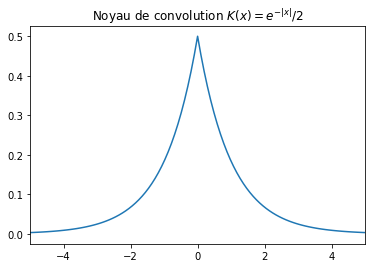
\includegraphics[scale = 0.6]{noyau.png}

Fig 1. Noyau
\end{center}

\subsection{Présentation}
\indent D'un point de vue concret, ce nouvel opérateur peut être interprété de la sorte : si $u(t,x)$ correspond à la densité de population en $x$ à l'instant $t$, alors on peut dire que la valeur $K(x-y)$ correspond à la probabilité de passer de $x$ à $y$ en un instant, et donc le terme $-u + K*u$  représente le taux en l'instant $t$ de population se déplaçant en $x$. Ainsi, cet opérateur est non local au sens que la convolution entraine que la diffusion au voisinage de $x$ ne dépend pas que des valeurs de $u(x,t)$ sur ce voisinage mais des valeurs de $u(x,t)$ partout ailleurs. 

Cette équation partage quelques propriétés communes avec l'équation de la chaleur $\partial_t u = d\partial_{xx}u$, par exemple les solutions stationnaires bornées sont constantes, mais aussi quelques différences : la diffusion non locale ne régularise pas les solutions en général. Un étude approfondie de l'équation sans terme de réaction a été effectuée dans l'article de Chaseigne, où il montre des résultats sur le comportement asymptotique des solutions de ce modèle de diffusion non local $\partial_t u = K*u - u$.


\subsection{Solution fondamentale}
\indent Nous allons rappeler brièvement les étapes pour avoir une solution de $(4)$ sans terme de réaction, et avec comme condition initale $u(0,x)=u_0(x)$. On suivra la démarche effectuer par Chaseigne via les transformées de Fourier. \newline

\noindent Il nous faut d'abord calculer la solution fondamentale qui correspond à la solution vérifiant :

\begin{equation*}
\left\{
  \begin{array}{cc}
\partial_t w(t,x) =  d(-w(t,x) + K*w(t,x)) \\
w(t=0,x) = w_0(x) = \delta_0(x)
\end{array}
\right.
\end{equation*}

\noindent où $\delta_0(x)$ est la distribution de dirac en 0, telle que $\int_{-\infty}^{\infty} \delta_0(x)dx = 1$

En passant l'équation en transformée de Fourier, on a donc :

\begin{equation*}
\left\{
  \begin{array}{cc}
\partial_t \widehat{w}(t,\xi) = d(-\widehat{w}(t,\xi) + \widehat{K}(\xi) \widehat{w}(t,\xi))\\
\widehat{w}(t=0,\xi) = 1
\end{array}
\right.
\end{equation*}

On a, pour $\xi$ fixé, une équation différentielle linéaire, dont la solution s'exprime par :

\begin{equation*}
\widehat{w}(t,\xi) = e^{d(\widehat{K(\xi)} -1)t}
\end{equation*}

et donc $w(x,t) = \mathcal{F}^{-1} (e^{d(\widehat{K(\xi)} -1)t})$\newline 

Enfin, on peut calculer toutes les autres solutions pour des certains $u_0$ avec cette solution fondamentale :

\begin{equation}
u(x,t) = w*u_0(x)
\end{equation}



\section{Solutions sous formes d'ondes}
Pour revenir à notre problème initial, on s'intéressera plûtot à l'équation $(4)$.

\subsection{Existence}
Dans le problème de l'équation de réaction diffusion avec opérateur laplacien, on avait remarqué qu'il existait des solutions sous forme d'ondes progressives. L'objectif est de savoir si il existe toujours de telles solutions dans le cas où la diffusion est non locale.

On veut donc trouver des solutions de la forme $u(t,x) = U(x-ct) $, pour une certaine volicité de propagation $c$ et avec $U(-\infty) = 0$ et $U(+\infty) = 1$. Autrement dit, on cherche un couple $(U,c)$ vérifiant l'équation :

\begin{equation}
\left\{
\begin{array}{cc}
0 = -U + K*U + cU' + f(U) \\
U(+\infty) = 0 , U(-\infty) = 1
\end{array}
\right.
\end{equation}

\noindent dans le cas où $d=1$.
Et un tel couple existe, avec en plus $u$ monotone. Cela a été démontré par Bates en 1997. On a même réussi à avoir des informations sur le comportement des solutions. Tout d'abord définissons la fonction suivante : 

\begin{equation}
	g(u,a,d) = u - \frac{1}{d} f(u)
\end{equation}
ce qui correspond au produit de convolution $K*u$ dans le cas où $c=0$. De plus, en supposant que $g$ a au plus trois intervalles de monotonie c'est à dire que :
\begin{equation*}
g'>0 \text{ sur } [0,\beta[\cup]\gamma,1], \text{ et } g'<0 \text{ sur } ]\beta,\gamma[
\end{equation*}
on peut définir pour $k \in \{ g(u,a,d), u \in [0,\beta[\} \cap \{ g(u,a,d), u \in ]\gamma, 1]\}$, la fonction : 
\begin{equation*}
	g_k(u,a,d) = \left \{ \begin{array}{cc} g(u,a,d), \text{ si } u \in  [0,\beta_1[\cup]\beta_2,1] \\ k , \text{ si } u \in [\beta_1,\beta_2] \end{array} \right.
\end{equation*}

\noindent où $g(\beta_1,a,d) = g(\beta_2,a,d) = k$, $\beta_1 \in [0,\beta]$ et $\beta_2 \in [\gamma,1]$. On peut alors énoncé le résultat de Bates.

\begin{Theoreme}[Bates 97]
	Soit $(u,c)$ solution de (7) alors : 

	(i) si $c \neq 0 $ alors $u \in \mathcal{C}^2$

	(ii) $c=0$ si et seulement si il existe un $k$ tel que $\int_0^1 g_k(u,a,d)du = \frac{1}{2}$

	(iii)  dans le cas où $c=0$, la solution $u$ a au plus un point de discontinuité. 
\end{Theoreme}

Ce théorème va entrainer de nombreuses conséquences dont les phénomène de blocages.

\subsection{Phénomènes de blocages}

Grâce au théorème 3.1, on peut remarquer dans certains cas, que les solutions sous forme d'onde ont tendance à se "stopper" et à faire apparaitre des discontinuités : c'est ce qu'on appelle des phénomènes de blocages. Ces phénomènes de blocages ont ainsi lieu dans une certaine région continue du $(d,a)$-espace que l'on sait bien décrire grâce au théorème de Bates. Cette question a été traitée notamment par les étudiants ayant participé au stage de recherche organisé aux états-unis par G. Faye. Dans (Fig.2), voici la zone théorique (situé en dessous de la courbe jaune), où il y a phénomène de blocage dans le cas où $f(u) = u(1-u)(u-a)$.

\begin{center}
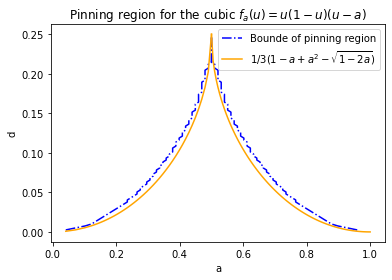
\includegraphics[scale = 0.6]{Pinning region.png}

Fig 2. Région où a lieu le phénomène de blocage
\end{center}

\section{Phénomène de seuil} 
On veut montrer, de la même manière que ce qui a été fait pour la diffusion laplacienne, l'existence d'un seuil $\ell *$ tel qu'on ait l'alternative :

$\cdot~ \forall \ell < \ell^* , u(t,x) \underset{t \to +\infty}{\overset{unif}{\longrightarrow}}0$ (Extinction)

$\cdot ~\forall \ell > \ell^* , u(t,x) \underset{t \to +\infty}{\overset{loc. unif}{\longrightarrow}}1$ (Propagation)

$\cdot$ et pour $\ell = \ell^* $ , $u(t,x) \underset{t \to +\infty}{\overset{unif}{\longrightarrow}}U_{*}(x)$ (Ground state)

\noindent où $U_*$ est l'unique solution de l'équation $U'' + f(U) = 0$ avec $U(\pm \infty) = 0$ et $ 0 \le U \le 1 $. Cette fonction que l'on présentera plus tard, a été étudié dans un article de Chmaj. 

\subsection{Existence de $\ell_0$}

Commençons, par analogie avec le cas du laplacien, par montrer l'existence de $\ell_0>0$ tel que $\forall \ell < \ell_0 , u(t,x) \underset{t \to +\infty}{\overset{unif}{\longrightarrow}}0$ (Extinction). \newline

Tout d'abord, énonçons un principe de comparaison, dans le contexte de notre problème : \newline
\begin{Theoreme}
Soient $f$ bistable, $K$ un noyau vérifiant $(5)$ et $v,w \in [0,1]$ tels que :

\begin{equation*}
\partial_t v - d(K*v - v) - f(v) \geq \partial_t w - d(K*w - w) - f(w)
\end{equation*}

Supposons que  $v(0,\cdot) \ge w(0,\cdot)$. Alors $v \ge w$.
\end{Theoreme}

Une version de ce théorème (plus forte) est démontrée dans l'article de .....\newline

Dans le contexte de la diffusion laplacienne, on avait une condition suffisante sur $u$ qui permettait de savoir si ce dernier convergeait uniformément vers 0. Il se trouve que cette condition reste vraie pour la diffusion non-locale. Pour le montrer, nous allons faire la même démarche que dans l'article de Aronson et Weinberger, même si les démonstrations sont très différentes. Voici le théorème : \newline

\begin{Theoreme}
Soit $\gamma \in [0,a[$ , les solutions de l'équation $(4)$ telles que $\forall x \in \mathbb{R}, u_0(x) \in [0,\gamma] $ vérifient :
\begin{equation*}
u(t,x) \underset{t \to +\infty}{\overset{unif}{\longrightarrow}}0
\end{equation*}
\end{Theoreme}
Pour montrer ce théorème, nous allons d'abord démontrer le lemme suivant : \newline 

\begin{Lemme}
Soit $f$ bistable, et $K$ vérifiant H1. Alors $\forall \gamma \in [0,a[$ , la solution $v(t,x)$ au problème de Cauchy :
\begin{equation}
\left\{
\begin{array}{cc}
\partial_t v (t,x) = & d(-v(t,x) + K*v(t,x)) + f(v(t,x))\\
v(0,x) = \gamma
\end{array}
\right.
\end{equation}

\noindent décroit vers 0 uniformément en $x$ lorsque $t \rightarrow +\infty$.
\end{Lemme}

\noindent \textit{Démonstration 4.3} : Dans le cas linéaire, $v(t,x) = w*v_0(x) = \gamma $ donc $v(t,x)_x = 0$. De plus, comme dans l'ont fait remarquer Aronson et Weinberger dans leur article, les solutions d'une telle équation sont toutes indépendantes de $x$. Posons alors $v(t,x) =\gamma(t) $. L'équation devient : 

\begin{equation*}
\begin{split}
\gamma '(t) & = d(-\gamma(t) + K*\gamma(t)) +  f(\gamma(t)) \\
& = d(-\gamma(t) + \int_{\mathbb{R}}K(y)\gamma(t)dy) +  f(\gamma(t)) \\
& = f(\gamma(t))
\end{split}
\end{equation*}

On obtient alors une équation différentielle autonome, et le portrait de phase de cette équation nous permet de conclure que $\gamma(t) \underset{t \to +\infty}{\longrightarrow}0$ et donc cela conclut le lemme. $\square$ \newline 

\noindent Le théorème 4.2 se démontre alors en utilisant ce lemme avec le principe de comparaison. \newline 

Maintenant, on veut utiliser ce résultat pour démontrer l'existence de $\ell_0$. Il s'agit donc de montrer qu'à partir d'une certaine valeur de $\ell$, on est sûr que notre solution sera dans $[0,a[$ à partir d'un certain t, et donc y restera et convergera uniformément vers 0. Nous avons réussi à démontrer ce résultat dans le cas où $f(u) = u(1-u)(u-a)$, avec $a \in ]0,1[$, ainsi que $K(x) = \frac{e^{-|x|}}{2}$, mais sous une certaine contrainte pour le coefficient de diffusion $d>0$. \newline 

\begin{Theoreme}[Théorème d'existence de $\ell_0$]Soient $\ell>0$ et $u$ solution de l'équation :
\begin{equation}
\left\{
  \begin{array}{cc}
   \partial_t u(t,x) =&  d(-u(t,x)+K*u(t,x))+f(u(t,x)) \\
   u(0,x) = & \mathds{1}_{[-\ell,\ell]}(x)~~~~~~~~~~~~~~~~~~~~~~~~~~~~~~~~~~~~~~~~~~~~~~~
   \end{array}
   \right.
   \end{equation}
Si $d > \frac{(1-a)^2}{4}$ , alors il existe $\ell_0 > 0$ tel que pour tout $\ell<\ell_0$, on a $u(t,x) \underset{t \to +\infty}{\overset{CU}{\longrightarrow}}0$. \end{Theoreme}


Avant de démontrer ce théorème, il sera utile de rappeler la solution fondamentale de l'équation de diffusion non locale dans notre contexte. Reprenons la relation $(6)$.
  	
Un simple calcul donne, pour $K(x) = \frac{e^{-|x|}}{2} $, d'une part, que $\widehat{K}(\xi) = \frac{1}{1+\xi^2}$ et donc on obtient $w(t,x) = \frac{1}{2\pi} \int_{\mathbb{R}} e^{d(\frac{1}{1+\xi^2}-1)t} e^{ix \xi} d\xi$. On peut même simplifier cette transformée inverse en utilisant la relation $e^{d(\frac{1}{1+\xi^2}-1)t} = e^{-dt} + (e^{\frac{dt}{1+\xi^2}}-1)e^{-dt}$ et en déduire que :

\begin{equation}
\begin{split}
\frac{1}{2\pi} \int_{\mathbb{R}} e^{d(\frac{1}{1+\xi^2}-1)t} e^{ix \xi} d\xi & = \frac{1}{2\pi} \int_{\mathbb{R}} (e^{-dt} + (e^{\frac{dt}{1+\xi^2}}-1)e^{-dt}) e^{ix \xi} d\xi \\ 
& = \frac{1}{2\pi} \int_{\mathbb{R}} e^{-dt}e^{ix\xi} d\xi + \frac{1}{2\pi} \int_{\mathbb{R}}(e^{\frac{dt}{1+\xi^2}}-1)e^{-dt} e^{ix \xi} d\xi \\ 
& = \frac{1}{2\pi} e^{-dt}\delta_0(x) + z(t,x)
\end{split}
\end{equation}

\noindent où $z(t,x) = \frac{e^{-dt}}{2\pi} \int_{\mathbb{R}}(e^{\frac{dt}{1+\xi^2}}-1) e^{ix \xi} d\xi$.

\noindent Nous avons désormais tous les outils pour démontrer le théorème 4.4.\newline

\noindent \textit{Démonstration 4.4} :La preuve se fait en trois étapes : \newline

\noindent \textbf{Etape 1 :} Majoration de la solution par une solution annexe.

Posons $c = \underset{u \in ]a,1[}{\text{sup} \{\frac{f(u)}{u}}\}$. On peut voir avec un calcul élémentaire que $  c = \frac{(1-a)^2}{4} $. Soit maintenant $v(t,x)$ la solution du problème de Cauchy suivant : 
\begin{equation*}
\left\{
  \begin{array}{cc}
    \partial_t v(t,x) =& d(-v(t,x) + K*v(t,x)) + cv(t,x) \\
    v(0,x) =& u_0(x) 
  \end{array}
  \right.
\end{equation*}

On voit par principe du maximum, que nécéssairement $v\ge 0$. De plus, par définition de $c$, et comme $f$ est négative sur $[0,a]$, on a que : 
\begin{equation*}
f(u) \le cu, ~~~~~~~~~~\forall u \in [0,1]
\end{equation*}

Ainsi, on peut en déduire que pour $u$ solution de l'équation : 

\begin{equation*}
\partial_t u - d(-u+K*u) +cu \le \partial_t u - d(-u+K*u) +f(u) = 0 
\end{equation*}

Or, $\partial_t v - d(-v + K*v)+- cv = 0$, donc on a que : 
\begin{equation*}
\partial_t v- d(-v + K*v) +cv \ge \partial_t u - d(-u+K*u) +cu 
\end{equation*}

et donc $v \ge u$ par principe de comparaison.\newline 

\noindent \textbf{Etape 2 :} Identification de $v$

Considérons $v(t,x) e^{-ct}$. On a que :
\begin{equation*}
\begin{split}
\partial_t(v(t,x) e^{-ct}) & = \partial_t v(t,x) e^{-ct} - c v(t,x)e^{-ct} \\
& = (d(-v(t,x) + K*v(t,x)) + cv(t,x))e^{-ct}  - c v(t,x)e^{-ct} \\
& = d(-v(t,x)e^{-ct} + K*v(t,x)e^{-ct})
\end{split}
\end{equation*}

Autrement dit, $v(t,x) e^{-ct}$ est solution de l'équation de diffusion non locale avec comme condition initiale $u_0$. Ainsi, grâce à la remarque préliminaire, on obtient que : 
\begin{equation*}
\begin{split}
  v(t,x) e^{-ct}& = w(t,.)*u_0(x)\\
  & = \int_{\mathbb{R}}\frac{\delta_0(x-y)e^{-td}}{2\pi}u_0(y)dy + \int_{\mathbb{R}}z(t,x-y)u_0(y)dy \\
  & = \frac{u_0(x)e^{-td}}{2\pi} + \int_{-l}^l z(t,x-y)dy
\end{split}
\end{equation*}

\noindent \textbf{Etape 3 :} Recherche de $l_0$

Maintenant nous allons majorer notre expression de $v$ pour obtenir une condition sur $l$ suffisante pour que $u$ tende uniformément vers $0$.


\begin{equation*}
\begin{split}
   |u(t,x)| \le |v(t,x)| & = |\frac{u_0(x)e^{t(c-d)}}{2\pi} + e^{tc}\int_{-l}^l z(t,x-y)dy|\\
   & \le \frac{e^{t(c-d)}}{2\pi} + e^{tc} \times|\int_{-l}^l \frac{e^{-dt}}{2\pi} \int_{\mathbb{R}}(e^{\frac{dt}{1+\xi^2}}-1) e^{i(x-y) \xi} d\xi dy| \\
   & \le \frac{e^{t(c-d)}}{2\pi}+ \frac{e^{t(c-d)}}{2\pi} \times\int_{-l}^l |\int_{\mathbb{R}}(e^{\frac{dt}{1+\xi^2}}-1) e^{i(x-y) \xi} d\xi |dy \\
\end{split}
\end{equation*}

Or, on voit que $ |\int_{\mathbb{R}}(e^{\frac{dt}{1+\xi^2}}-1) e^{ix \xi} d\xi | \le \int_{\mathbb{R}}(e^{\frac{dt}{1+\xi^2}}-1) |e^{ix \xi}| d\xi =\int_{\mathbb{R}}(e^{\frac{dt}{1+\xi^2}}-1)d\xi $, une intégrale qui converge pour tout $t>0$. On pose alors $M_t>0$ cette intégrale. On obtient alors : 

\begin{equation*}
\begin{split}
|u(t,x)| & \le \frac{e^{t(c-d)}}{2\pi}(1+\int_{-l}^l |\int_{\mathbb{R}}(e^{\frac{dt}{1+\xi^2}}-1) e^{i(x-y) \xi} d\xi |dy) \\
& \le \frac{e^{t(c-d)}}{2\pi}(1+2lM_t)
\end{split}
\end{equation*}

Ainsi, par le théorème 4.2, $u$ va converger uniformément vers 0 dès que $\frac{e^{t(c-d)}}{2\pi}(1+2lM_t) <a$, soit lorsque $l < \frac{2\pi a e^{t(d-c)}-1}{2M_t}$. Cependant, on souhaite $l>0$, on a donc la suivante condition sur le membre de droite pour que $l$ existe : $2\pi a e^{t(d-c)}>1$ condition qui sera vérifié pour un certain temps $t_0>0$ si $d>c$. Ainsi, en posant $l_0 =  \frac{2\pi a e^{t_0(d-c)}-1}{4M_{t_0}}$, le théorème est prouvé. $\square$ \newline 


On a donc bel et bien existence d'un $\ell_0>0$ dans une certaine région du plan $(a,d)$. Une question légitime est de savoir ce qu'il se passe sous cette région. Regardons une simulation pour développer notre intuition. Voici une solution numérique (Fig.3) dans le cas où il y a propagation (hors pinning) dans le cas où $d<\frac{(1-a)^2}{4}$ :  

\begin{center}
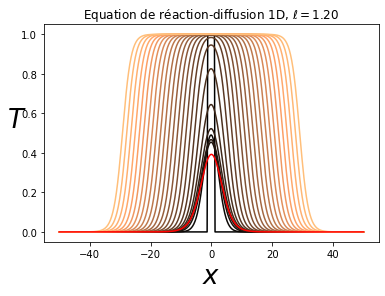
\includegraphics[scale = 0.6]{propagation.png}

Fig. 3 Propagation pour $d = 0,1$, $a = 0,35$ et $l=1,9$
\end{center}

Ici, on voit sans surprise qu'il semblerait y avoir existence d'un $\ell_1>0$ comme pour le cas laplacien. Par contre, si on se place avec un $\ell>0$ assez petit, nous avons observé qu'il n'y a pas d'extinction pour les mêmes valeurs de $a$ et $d$ (Fig. 4). Il n'y a pas de convergence uniforme en 0 (ni même de convergence dans $L^{\infty}$). 

\begin{center}
\includegraphics[scale=0.6]{sort	of ground state.png}

Fig. 4 Pas d'extinction pour $d = 0,1$, $a = 0,35$ et $l=0,5$
\end{center}

Cependant, cet absence de seuil pour l'extinction laisse place à un autre totalement différent : il semblerait que le seuil ne sépare pas la propagation de l'extinction, mais plutôt d'une zone de solution de type "ground state".


\subsection{Ground State}

















\end{document}